\documentclass[12pt]{article}
\usepackage{graphicx} % Required for inserting images

\usepackage[english]{babel}
\usepackage[letterpaper,top=2cm,bottom=2cm,left=3cm,right=3cm,marginparwidth=1.75cm]{geometry}

% Useful packages
\usepackage{amsmath}
\usepackage{graphicx}
\usepackage[colorlinks=true, allcolors=blue]{hyperref}

\title{COS710 - Artificial Intelligence 1: Assignment 3}
\author{Seale Rapolai - 15122116}
\date{May 2026}

\begin{document}
\maketitle

\section{Dataset} \label{sec:dataset}
    The dataset utilized is the Residential Energy Dataset UK (2014-2020). It contains continuous time-series observations of electricity load demand recorded over a 6-year period. Forecasting electricity consumption is a critical task for energy providers, often addressed through advanced computational methods such as Grammatical Evolution \cite{castelli2015}. The original data instances are captured at 15-minute intervals. Given that this is a time-series forecasting problem, past observations must be used to predict future instances. For this experiment, the dataset is restructured through a sliding window by creating lagged attributes; specifically, the models are trained utilizing $m=8$ contiguous previous values to predict the forthcoming electricity load.

    \subsection{Preprocessing}
    The dataset, supplied in CSV format, was loaded into a Python Pandas DataFrame. To maintain temporal integrity, the observations were sorted in ascending order based on the $utc\_timestamp$ column. $pandas.Timedelta$ was then used to verify that the time series was continuous, confirming a uniform 15-minute interval between consecutive data points with no missing entries.
    \\
    For the feature engineering phase, the $Electricity\_load$ column was isolated into a new DataFrame to serve as the target variable. To incorporate historical context, the $m$ lagged features were generated by applying shift operations. Specifically, for each $i \in [1, m]$, a new column $load_{t-i}$ was created to represent the electricity load at $t-i$. With $m$ set to 8, these features represent a sliding window of the previous two hours:
    \begin{itemize}
        \item $load_{t-1}$: Load from 15 minutes prior. 
        \item $load_{t-2}$: Load from 30 minutes prior
        \item Up to $load_{t-8}$ (120 minutes prior).
    \end{itemize}

    As a consequence of the shift operations, the initial rows of the dataset contained $null$ values where historical data was unavailable. These incomplete rows were removed to ensure a clean dataset for subsequent analysis.

\section{Performance metric}
    The performance metric used to assess the quality of the algorithmic predictor is the \textbf{Mean Absolute Percentage Error (MAPE)}.
    
    \textbf{How it works:} MAPE mathematically computes the average absolute percentage difference between the estimated values produced by the decoded phenotype expression tree and the actual known electricity load values in the fitness cases.
    
    \textbf{Why it was chosen:} It is one of the most robust evaluators for numeric regression problems dealing with shifting temporal datasets. Unlike MSE, MAPE provides a scale-invariant metric that prevents the fitness score from being distorted by the naturally fluctuating variance across different seasonal consumption cycles.

\section{Standard Grammatical Evolution (GE)}

    To enforce structural constraints on the evolved predictive models, this assignment utilizes \textbf{Standard Grammatical Evolution (GE)} \cite{oneill2001}.

    GE decouples the evolutionary search space from the physical expression space by maintaining a dual representation:
    \begin{itemize}
        \item \textbf{Genotype:} A single flat list of integer codons (typically in the range $[0, 255]$). These codons are used to select expansion rules sequentially during the parsing process.
        \item \textbf{Phenotype:} An executable mathematical expression tree generated by recursively parsing the genotype using a context-free grammar.
    \end{itemize}
    
    Parsing begins at the start symbol of the grammar. At each step, the next non-terminal is expanded by retrieving the next codon in the flat list and choosing the production rule index using a modulo operator: 
    \begin{equation}
        \texttt{Rule Index = codon \% Number Of Rules For Non Terminal}
    \end{equation}
    
    If the codon list is exhausted before the derivation terminates, the reading pointer wraps around back to the beginning of the genotype list. A maximum wrap-around limit of $10$ wraps (or a maximum node limit of $1000$) is enforced to prevent infinite loops. Individuals exceeding these limits are declared invalid and assigned a high penalty fitness value of $10^9$.

\section{Representation, Terminal Sets, and Function Sets}
    The solution uses a grammar-defined symbolic representation. The Backus-Naur Form (BNF) grammar maps the flat search space of integer codons to syntax trees, maintaining the mathematical order of operations while ensuring that the resulting equations are transparent and human-interpretable.

    The Context-Free Grammar (CFG) used in this assignment is defined below:
    \begin{align*}
        \langle\text{root}\rangle &::= \text{StructuredRoot}(\langle\text{expr}\rangle, \langle\text{expr}\rangle) \\
        \langle\text{expr}\rangle &::= \text{Function}(\langle\text{op}\rangle, \langle\text{expr}\rangle, \langle\text{expr}\rangle) \mid \text{Variable}(\langle\text{var}\rangle) \mid \text{Constant}(\langle\text{const}\rangle) \\
        \langle\text{op}\rangle &::= + \mid - \mid \times \mid \div \mid \text{max} \mid \text{min} \\
        \langle\text{var}\rangle &::= load_{t-1} \mid load_{t-2} \mid load_{t-3} \mid load_{t-4} \mid load_{t-5} \mid load_{t-6} \mid load_{t-7} \mid load_{t-8} \\
        \langle\text{const}\rangle &::= C
    \end{align*}

    \subsection{Terminal set:}
    The terminals consist of the $m=8$ contiguous lagged values extracted from the historical sliding window (i.e., $load_{t-1}$ to $load_{t-8}$), combined with an ephemeral random constant $C$ to inject variance.
    \begin{itemize}
        \item $load_{t-i}$: Electricity load at $i$ previous time steps, for $i \in [1,8]$.
        \item $C$: An ephemeral constant value derived directly from the codon value using Equation \ref{eq:const_equation}, yielding coefficients cleanly in the range $[-0.2, 0.2]$.
        \begin{equation}
            C = \text{round}(((codon \% 256) / 255.0) * 0.4 - 0.2, 2)
            \label{eq:const_equation}
        \end{equation}
    \end{itemize}
    
    \subsection{Function set:}
    The set consists of basic arithmetic primitives and threshold operators configured as binary functions, with an arity of 2:
    \begin{itemize}
        \item Arithmetic operators: Addition ($+$), Subtraction ($-$), Multiplication ($\times$), and safe Division ($\div$, which returns 1 when the denominator is zero).
        \item Threshold operators: Minimum ($\text{min}$) and Maximum ($\text{max}$), which capture peak energy loads and seasonal demand limits.
    \end{itemize}

    Equation \ref{eq:predictor1} below shows an example of a decoded phenotype formula:
    \begin{equation}
        \hat{y}_t = \text{StructuredRoot}(\text{min}(load_{t-2}, load_{t-1}) + (-0.12 \times -0.04))
        \label{eq:predictor1}    
    \end{equation}

    Figure \ref{fig:sample_tree} visualizes the phenotype structure corresponding to Equation \ref{eq:predictor1}.
    \\
    \begin{figure}[!ht]
        \centering
        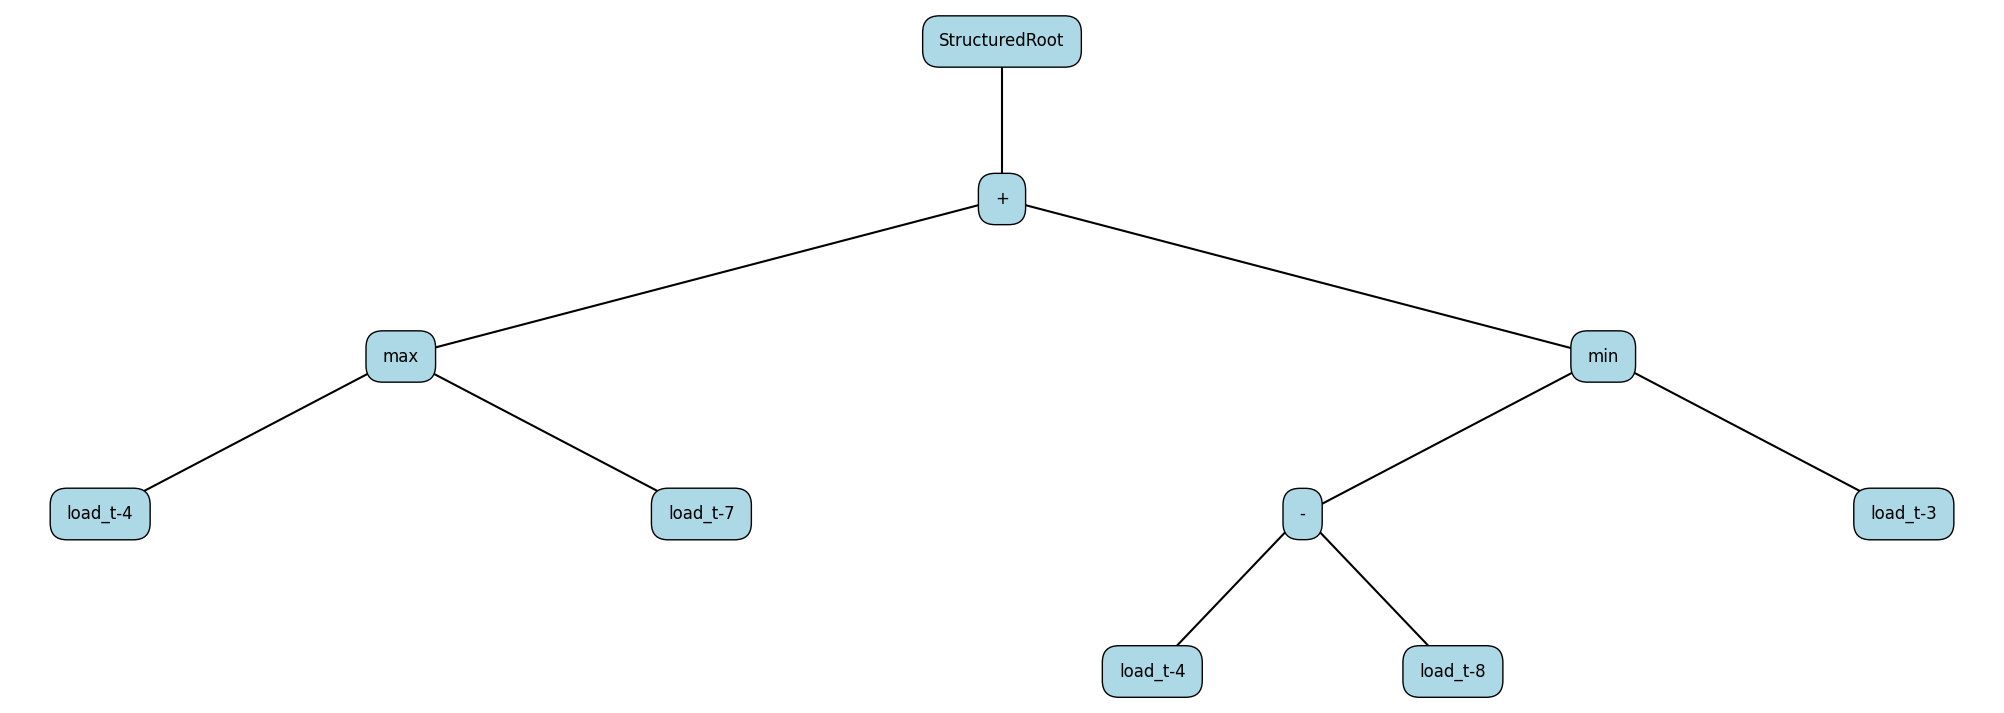
\includegraphics[width=0.9\textwidth]{sample_tree.png}
        \caption{Example phenotype tree representing a grammar-derived individual.}
        \label{fig:sample_tree}
    \end{figure}
    
\section{Initial population generation}
    The initial population is generated using \textbf{Sensible Initialisation} in association with the \textbf{Ramped Half-and-Half} method \cite{poli2008} to guarantee valid initial genotypes.
    
    For a given population size, the derivation process employs a 50/50 split between two creation strategies:
    \begin{itemize}
        \item \textbf{Full method:} During the recursive grammar derivation, if the current depth is strictly less than the target depth, the expansion rule is locked to index $0$ (\texttt{Function}). This forces the tree to grow until it reaches the maximum depth limit, where it terminates.
        \item \textbf{Grow method:} While the current depth is less than the target depth, the rule index is selected completely at random from all valid production rules (\texttt{Function}, \texttt{Variable}, or \texttt{Constant}), allowing branches to terminate early and produce asymmetrical trees.
    \end{itemize}

    Once the target depth is reached, rule selection is restricted to terminal options (Variable or Constant) to force termination. To map these derivations to the flat list representation, the selected rule indices are mapped to codon values (\texttt{codon \% len(rules) == r\_idx}), generating a standard flat integer array of standard 8-bit integers ($[0, 255]$).

\section{Fitness}
    \subsection{Fitness Cases}
    The algorithm evaluates individuals across a dynamic sliding window extracted from the time-series dataset. A batch window (representing a specific number of days, governed by the \texttt{window-size} argument) is selected. Each row within this temporal slice acts as a single fitness case, offering the 8 lagged input variables ($load_{t-1}$ to $load_{t-8}$) and the target \verb|Electricity_load|. The window shifts forward every generation, ensuring the population learns to generalize across seasonal consumption shifts instead of overfitting to a static dataset.
    
    \subsection{Fitness Evaluation}
    During evaluation, each individual's integer genotype is decoded into an executable phenotype expression tree. The raw fitness is computed using the scale-invariant \textbf{Mean Absolute Percentage Error (MAPE)}.
    
    The exact fitness function $F(T)$ for a decoded phenotype tree $T$ evaluated over $N$ fitness cases is defined in Equation \ref{eq:mape}:
    \begin{equation}
        F(T) = \frac{1}{N} \sum_{i=1}^{N}
        \begin{cases} 
          10 & \text{if } T(x_i) \text{ results in an exception} \\
          \left| \frac{y_i - T(x_i)}{\max(|y_i|, 10^{-8})} \right| & \text{otherwise}
       \end{cases}
       \label{eq:mape}
     \end{equation}
    where $N$ is the number of fitness cases, $x_i$ is the input lagged vector, $T(x_i)$ is the model's predicted output, and $y_i$ is the actual target load.

    To ensure algorithmic stability and dynamic modeling, the evaluation pipeline includes three critical safeguards:
    \begin{enumerate}
        \item \textbf{Denominator Bounding:} The term $\max(|y_i|, 10^{-8})$ prevents division-by-zero errors when the target load $y_i$ is zero or infinitesimally small. By clamping the denominator to a microscopic lower bound ($10^{-8}$), the function mathematically guarantees a finite MAPE score regardless of anomalous zero-values in the dataset.
        \item \textbf{Exception Handling:} If the phenotype equation triggers a mathematical exception (e.g., extreme overflow) on a specific test case $x_i$, that individual case is assigned a severe localized penalty of $10$ (equivalent to a 1000\% error). This aggressively discourages mathematically unstable structures.
        \item \textbf{Structural Parsimony Pressure:} To prevent the algorithm from finding a trivial static optimum (constant bloat) and to explicitly control unchecked code growth \cite{luke2006}, the fitness evaluator actively inspects the phenotype tree structure prior to calculation. If the decoded equation is entirely devoid of lagged \texttt{Variable} nodes (e.g., it is a flat baseline constant), it is immediately rejected and assigned a penalty MAPE of $1.0$. This ensures the evolutionary process is strictly forced to model dynamic relationships instead of settling on safe averages.
    \end{enumerate}
    
    Finally, if an individual fails the parsing phase entirely (e.g., by exceeding the grammar wrap-around limit and failing to produce a valid tree), it is immediately assigned an extreme global penalty of $10^9$. Because the evolutionary loop actively minimizes $F(T)$ toward zero, these penalty mechanisms guarantee that invalid and structurally unstable genotypes are swiftly eliminated from the breeding pool.

\section{selection method} \label{sec:selection_method}
    The algorithm utilizes \textbf{Tournament Selection} \cite{miller1995} to select individuals for genetic operators. For each selection event, the algorithm samples a uniform subset of individuals from the population (defined by the \verb|tournament-size| parameter). These candidates compete, and the individual with the lowest phenotype MAPE wins the tournament and is passed to the genetic operators.
    
    Tournament selection provides several key advantages:
    \begin{enumerate}
        \item \textbf{Scale Independence:} By comparing only the relative rank within the tournament, the selection is immune to large fluctuations in absolute MAPE values across shifting seasonal windows.
        \item \textbf{Adjustable Selection Pressure:} Tuning the tournament size alters the convergence velocity. A small size (e.g., 2) maintains genetic diversity by allowing weaker genotypes to occasionally breed, whereas a larger size drives rapid convergence.
        \item \textbf{High Efficiency:} Selecting parents operates in $O(k)$ time (where $k$ is the tournament size), bypassing the computational overhead of global sorting.
    \end{enumerate}

\section{Genetic operators}
    The standard GE algorithm applies three core genetic operators at the genotype level to navigate the flat search space: \textbf{Crossover}, \textbf{Mutation}, and \textbf{Reproduction}. These operators are applied based on strict proportional rates.

    \begin{enumerate}
        \item \textbf{Reproduction (Elitism):} 
        The top percentage of the population is identified by sorting the fitness values. Their genotype lists are copied directly to the next generation without modification. This operator heavily promotes \textbf{exploitation}. By preserving the mathematically fittest models exactly as they are, it ensures the algorithm does not regress and safely maintains the best discovered solutions across generations.
   
        \item \textbf{Flat Genotype Crossover:}
        Two parents are chosen via Tournament Selection. A random single-point cut is chosen within their overlapping length, and their flat integer lists are recombined to generate two child genotypes. If the decoded children violate the global \verb|max_depth| constraint, the crossover is rejected and the parents are returned unaltered. This operator perfectly balances both search strategies. It \textbf{exploits} known fit sub-components by combining successful genetic sequences, while simultaneously \textbf{exploring} novel structural configurations in the phenotype tree. Additionally, rejecting invalid children safely curbs uncontrolled structural bloat.
    
        \item \textbf{Flat Genotype Mutation:} 
        Codon flip mutation is applied to a single parent: every codon has a 15\% chance of being replaced by a completely new random integer in $[0, 255]$. This seemingly high per-codon mutation rate is intentionally chosen to counteract the genetic redundancy inherent in Grammatical Evolution. Because multiple integers map to the same grammar rule via the modulo operator, many codon flips result in neutral mutations that do not alter the phenotype. The 15\% rate ensures that enough meaningful structural changes actually survive the mapping process to drive evolution. This operator acts as the primary engine for \textbf{exploration}, introducing entirely fresh genetic material into the population to prevent premature stagnation and escape local optima. Furthermore, fine-tuning is achieved organically during this exploratory phase, as mutating a constant codon directly shifts its derived floating-point coefficient.
    \end{enumerate}

    \subsection{Structural Similarity in Crossover}
    To prevent redundant crossover events that lead to local optima, the system implements morphological similarity tracking using two distinct indices computed on the decoded phenotype trees \cite{kapoor2023}:
    \begin{itemize}
        \item \textbf{Global Index (GI):} Measures the number of matching function nodes shared between two phenotypes from the root down to a cutoff depth limit (half of the maximum depth).
        \item \textbf{Local Index (LI):} Counts matching function and terminal nodes in the subtrees beyond the cutoff depth.
    \end{itemize}

\section{Experimental setup} \label{sec:exp_setup}
    \newcommand{\PopSize}{100}
    \newcommand{\NoGens}{70}
    \newcommand{\MaxDepth}{5}
    \newcommand{\FitnessFunc}{Mean Absolute Percentage Error (MAPE)}
    \newcommand{\TestCases}{30 days sliding window chunk offsets}
    \newcommand{\SMethod}{Tournament Selection}
    \newcommand{\TournSize}{2}
    \newcommand{\PopMethod}{Sensible Ramped half-and-half}
    \newcommand{\MRate}{19\% (19 individuals per 100)}
    \newcommand{\CRate}{80\% (80 individuals per 100)}
    \newcommand{\RRate}{1\% (1 individual per 100)}
    
    \textbf{Hardware specifications:} Intel(R) Core(TM) i7-8750H CPU @ 2.20GHz with 16 GB of RAM.
   
    Table \ref{tab:gp_parameters} lists the parameters applied during this simulation:
  
    \begin{table}[h]
        \centering
        \begin{tabular}{ll}
            \hline
            \textbf{Parameter} & \textbf{Value}\\
            \hline
            Population size & $\PopSize$ \\
            Max depth & $\MaxDepth$ \\
            Initial population generation & \PopMethod \\
            Fitness function & $\FitnessFunc$ \\
            Test Cases / Window Constraints & \TestCases \\
            Selection method & \SMethod \\
            Tournament Size & $\TournSize$ \\
            Mutation rate & \MRate \\
            Crossover rate & \CRate \\
            Reproduction Rate & \RRate \\
            Number of generations & $\NoGens$ \\
            Termination criteria & Fixed generation limit reached \\
            \hline
        \end{tabular}
        \caption{Standard GE configuration parameters}
        \label{tab:gp_parameters}
    \end{table}

    The parameters balance computational efficiency, search space traversal, and phenotypic interpretability:
    \begin{itemize}
        \item \textbf{Population Size (100) \& Max Depth (5):} Prevents tree bloat and ensures the evolved equations are lean, highly interpretable, and generalized.
        \item \textbf{Genetic Rates (80\% Crossover / 19\% Mutation / 1\% Elitism):} Maximizes constructive recombination while continuously introducing structural and constant-level variance.
        \item \textbf{Tournament Size (2):} Maintains diverse selection dynamics, allowing suboptimal but structurally novel individuals to breed.
        \item \textbf{Generations (70):} Explicitly calculated to cover the entire historical dataset (201,596 instances) over the sliding window length of 30 days (2,880 instances per generation):
        \begin{equation}
            \text{Generations} = \left\lceil \frac{\text{Total Instances}}{\text{Instances per Window}} \right\rceil = \left\lceil \frac{201,596}{2,880} \right\rceil \approx 70
        \end{equation}
    \end{itemize}

\section{Results}
    The Standard GE algorithm successfully converged across all experimental runs. The system demonstrated strong generalization capacities, navigating the tumbling sliding window that exposes the population to new temporal offsets every generation.
    
    \begin{table}[h]
        \centering
        \begin{tabular}{|c|c|c|}
            \hline
            \textbf{Run NO.} & \textbf{Random seed} & \textbf{Best Individual (MAPE)}  \\
            \hline
             1 & 35 & $0.1996$ \\
            \hline
             2 & 83 & $0.2008$ \\
            \hline
             3 & 75 & $0.2101$ \\
            \hline
             4 & 97 & $0.2107$ \\
            \hline
             5 & 14 & $0.2146$ \\
            \hline
             6 & 40 & $0.2150$ \\
            \hline
             7 & 66 & $0.2160$ \\
            \hline
             8 & 36 & $0.2187$ \\
            \hline
             9 & 89 & $0.2258$ \\
            \hline
             10 & 47 & $0.2348$ \\
             \hline
             \multicolumn{2}{|c|}{mean} & $0.2146$ \\
             \hline
             \multicolumn{2}{|c|}{Std. Div} & $0.0100$ \\
             \hline
        \end{tabular}
        \caption{Execution results for the best 10 runs}
        \label{tab:results}
    \end{table}

    As shown in Table \ref{tab:results}, across 10 independent experimental runs, the best individual consistently achieved a MAPE between \textbf{19.96\%} and \textbf{23.48\%}. The mean across all runs is \textbf{21.46\%}, with a narrow standard deviation of \textbf{1.00\%}, highlighting the algorithm's robustness across multiple independent runs with different random seeds.

    The best individual across all runs was found in \textbf{Run 1 (Seed 35)}, with a MAPE of \textbf{19.96\%}. The evolved phenotype heavily utilizes nested arithmetic and variable structures to model peak loads. Figure \ref{fig:best_indiv_35} illustrates this tree.
    \\
    \begin{figure}[!ht]
        \centering
        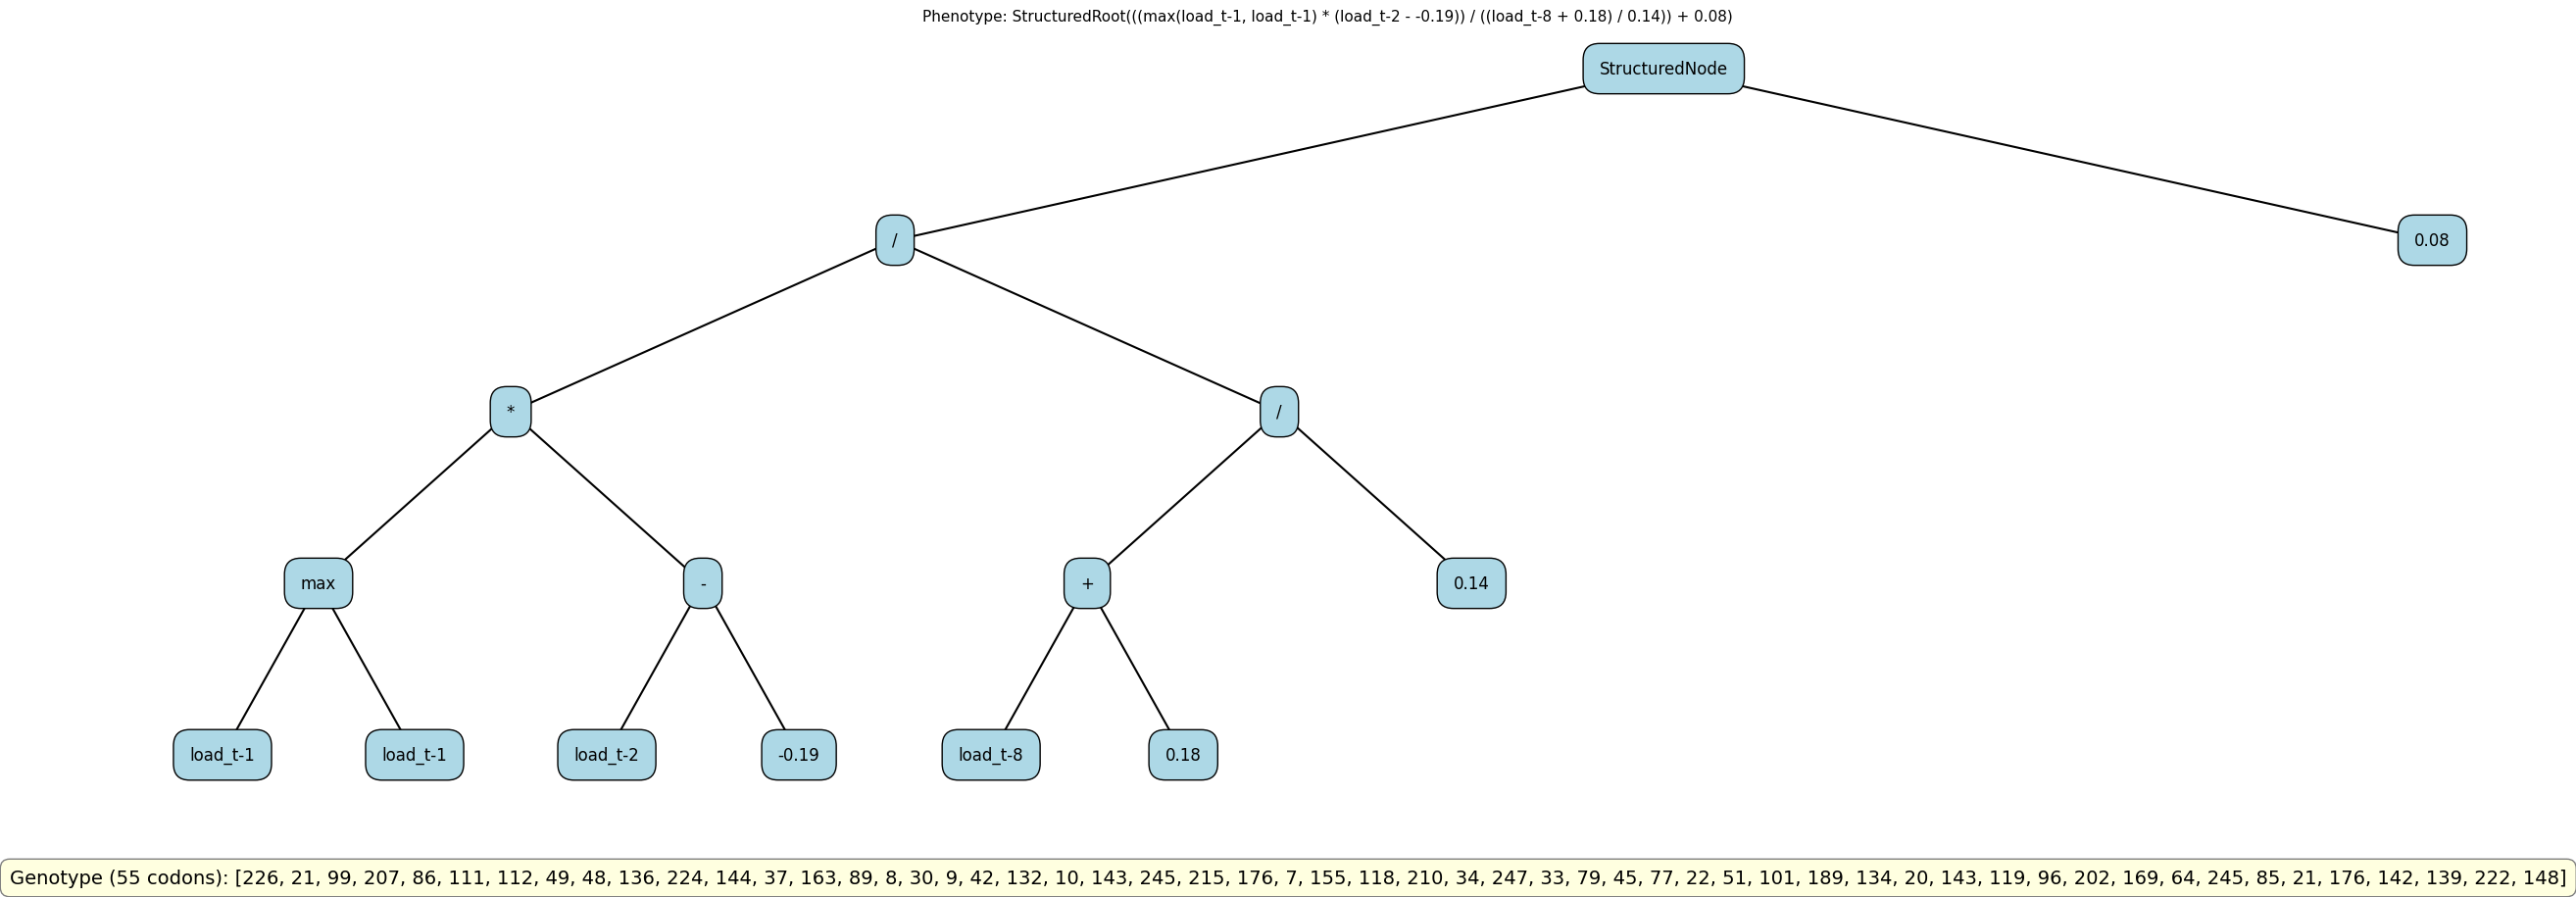
\includegraphics[width=0.95\linewidth]{35_individual_tree.png}
        \caption{Binary Expression Tree of the best individual from run 1, using 35 as random seed.}
        \label{fig:best_indiv_35}
    \end{figure}
    
    Due to the online sliding window, the algorithm experiences minor dataset shock at the start of each generation. However, the average and worst errors converge sharply as shown in Figure \ref{fig:gp_fitness_evolution}, crashing downward from extreme generation-0 outliers and squeezing tightly against the elite baseline.
    
    \begin{figure}[!ht]
        \centering
        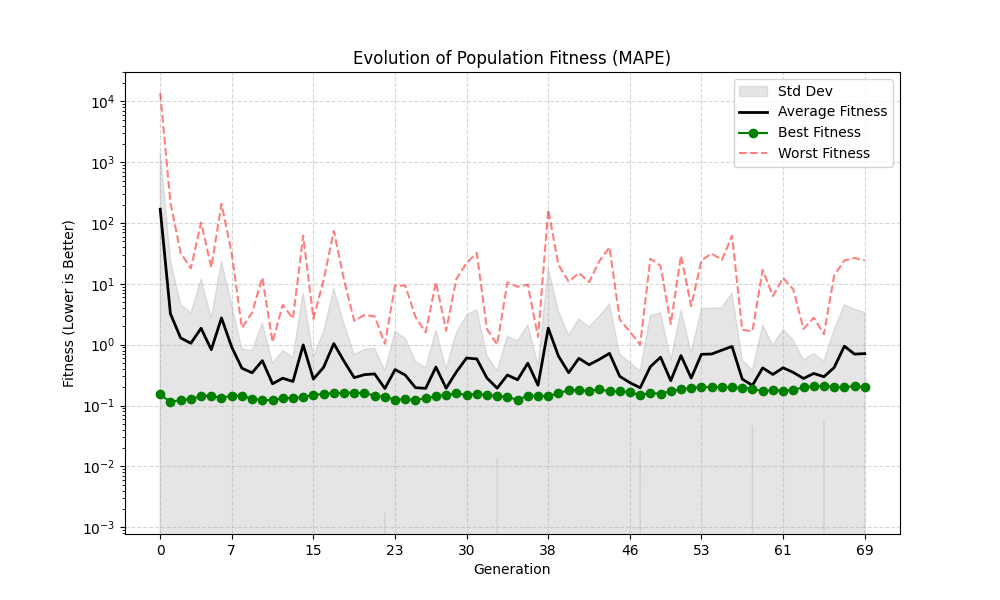
\includegraphics[width=0.98\linewidth]{20260524_200715_gp_fitness_35.png}
        \caption{Evolution of population fitness over generations.}
        \label{fig:gp_fitness_evolution}
    \end{figure}
    
    Figure \ref{fig:gp_best_fitness_evolution} exhibits minor fluctuations (bouncing between roughly 12\% and 20\% MAPE), which is an expected consequence of the tumbling sliding window. Every generation, the elite tree is evaluated on unseen data, reflecting shifting seasonal predictability. The stable elite MAPE confirms the discovery of highly generalized models that resist overfitting.
  
    \begin{figure}[!ht]
        \centering
        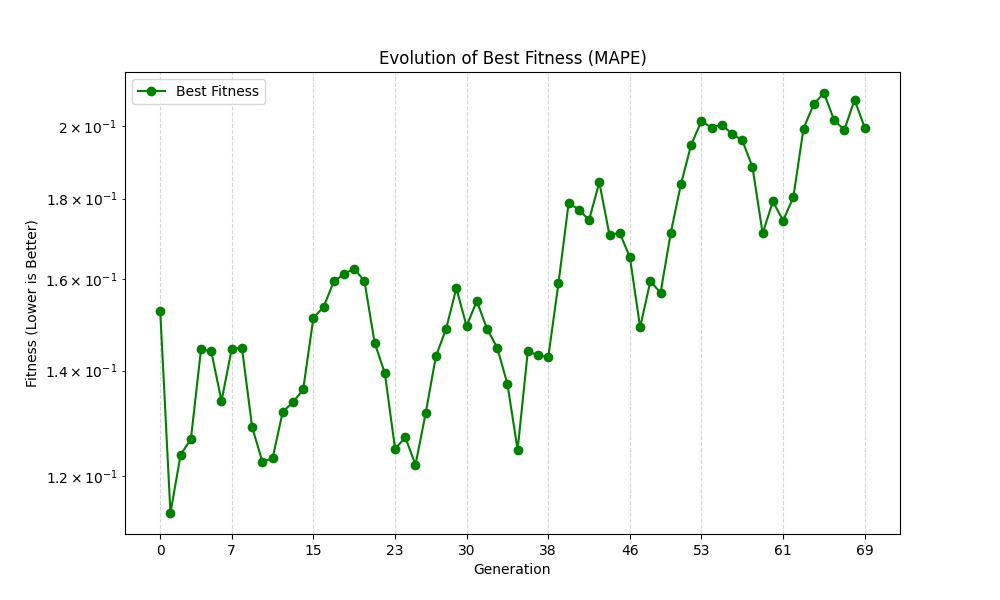
\includegraphics[width=0.95\linewidth]{20260524_200715_gp_best_fitness_35.png}
        \caption{Evolution of best individual's fitness per generation.}
        \label{fig:gp_best_fitness_evolution}
    \end{figure}

\section{Run times}
    To ensure computational scalability across the 5.7 years of temporal data, the fitness evaluation pipeline was fully refactored to utilize asynchronous multiprocessing, distributing the load of evaluating 100 individuals across all available CPU cores.

    Across the 10 experimental runs, processing 70 generations took between \textbf{870.32 seconds} (14.5 minutes) and \textbf{951.00 seconds} (15.8 minutes). On average, a complete traversal of the 201,596-row dataset took roughly \textbf{15.0 minutes}.

    \begin{table}[h]
        \centering
        \begin{tabular}{|c|c|c|}
            \hline
            \textbf{Run NO.} & \textbf{Random seed} & \textbf{Execution Time (Seconds)}  \\
            \hline
             1 & 35 & 888.09 \\
            \hline
             2 & 83 & 923.20 \\
            \hline
             3 & 75 & 924.04 \\
            \hline
             4 & 97 & 951.00 \\
            \hline
             5 & 14 & 884.55 \\
            \hline
             6 & 40 & 872.59 \\
            \hline
             7 & 66 & 870.32 \\
            \hline
             8 & 36 & 883.82 \\
            \hline
             9 & 89 & 876.71 \\
            \hline
             10 & 47 & 901.02 \\
              \hline
              \hline
              \multicolumn{2}{|c|}{\textbf{mean}} & 897.53 \\
              \hline
              \multicolumn{2}{|c|}{\textbf{Std. Div}} & 25.44 \\
              \hline
        \end{tabular}
        \caption{Execution results for the best 10 runs}
        \label{tab:runtimes}
    \end{table}

    The run times shown in Table \ref{tab:runtimes} prove that the algorithm successfully balances structural complexity with processing speed, maintaining a relatively lean tree architecture (Max Depth = 5) while computing tens of millions of mathematical operations across the feature set. The overall mean execution time of \textbf{897.53 seconds} (approximately 15.0 minutes) demonstrates highly efficient traversal of the 5.7-year dataset. The standard deviation of \textbf{25.44 seconds} indicates that the computational load is extremely stable across different random seeds, successfully mitigating the extreme processing variances commonly caused by uncontrolled tree bloat.

\section{Comparison of Previous Assignments}

    The fundamental evolution from Assignment 1 and 2 to Assignment 3 lies in the mechanism of structural enforcement: the transition from Genetic Programming (GP) to Standard Grammatical Evolution (GE). This architectural upgrade completely redefines how structural validity is maintained during the evolutionary process.

    \subsection{Context-Free Grammar as the Structural Core}
        In standard GP (Assignment 1) and Structure-Based GP (Assignment 2), the search space and the expression space were identical: operations were performed directly on the morphological trees. While Assignment 2 utilized a similarity index to manage structural diversity, it still relied on tree-based crossover which inherently risked creating invalid or bloated mathematical expressions if not strictly constrained.

        In contrast, Assignment 3 introduces the \textbf{Context-Free Grammar (CFG) and Genotype-Phenotype mapping} as its primary structural component. By decoupling the flat integer search space (genotype) from the executable trees (phenotype), GE offloads all structural responsibilities to the grammar.

    \subsection{Enforcing Structural Validity and Constraints}
        The grammar serves as an absolute structural blueprint. It explicitly enforces the order of operations, prevents mathematical type mismatches, and restricts the search space exclusively to valid equations. Because crossover and mutation occur on the flat integer lists, the genetic operators are completely agnostic to the phenotype structure. 
        
        However, the integrity of the resulting phenotype is mathematically guaranteed by the CFG during the decoding phase. This strict, decoupled structure mitigates the destructive crossover events seen in Assignment 1. Furthermore, while the GE architecture inherently manages structural validity, the algorithm strategically retains the morphological similarity tracking (Global and Local Indices) from Assignment 2 to prevent redundant crossover events, blending the structural safety of GE with the diversity-preservation of Structure-Based GP.

    \subsection{Comparison of Execution Metrics and Performance}
        The architectural differences between the three assignments directly impacted their convergence accuracy and computational efficiency.
        
        \textbf{Computational Efficiency and Run Times:} 
        Assignment 1 (Standard GP) suffered from unconstrained code growth (bloat) and expensive direct tree recombinations. It required approximately 12 to 13 minutes to simulate just 20 generations. Scaled to the 70 generations used in later assignments, it would be highly inefficient.
        Assignment 2 (Structure-Based GP) solved the bloat issue by introducing morphological similarity tracking (Global and Local Indices). While this allowed the system to simulate 70 generations in an average of \textbf{20.5 minutes}, the recursive tree-comparison algorithms introduced significant overhead.
        Assignment 3 (Standard GE) proved to be the most computationally efficient architecture, completing 70 generations in a mean time of just \textbf{15.0 minutes}. By shifting genetic operations (crossover and mutation) to flat integer arrays rather than recursive tree structures, the genetic operators execute in linear time. Although it retains the morphological similarity checks from Assignment 2 to prevent redundant crossover, the strict structural parsimony pressure limits tree bloat so effectively that the overhead of these similarity checks remains negligible, leading to massive overall execution speedups.

        \textbf{Predictive Accuracy (MAPE):} 
        Because Assignment 1 utilized Mean Squared Error (MSE), its raw fitness values cannot be directly compared to the latter iterations. However, Assignments 2 and 3 both utilize the Mean Absolute Percentage Error (MAPE) under identical tumbling window constraints. 
        Assignment 2 achieved a slightly superior mean MAPE of \textbf{19.10\%}, whereas Assignment 3 achieved \textbf{21.46\%}. This minor regression in accuracy is a known trade-off of Grammatical Evolution. Because GE utilizes an indirect genotype-to-phenotype mapping via modulo operations, a single point mutation in the integer array can drastically alter the decoding pathway of all subsequent codons (the ripple effect). This makes fine-tuning (exploitation) slightly harder in GE than in the direct tree-based mutations of Structure-Based GP, resulting in a marginally higher final error rate despite the massive gains in execution speed and structural safety.

\begin{thebibliography}{9}

\bibitem{kapoor2023}
Kapoor, R., \& Pillay, N. (2023). Iterative Structure-Based Genetic Programming for Neural Architecture Search. \textit{Proceedings of the Companion Conference on Genetic and Evolutionary Computation (GECCO '23 Companion)}, 595–598.

\bibitem{oneill2001}
O'Neill, M., \& Ryan, C. (2001). Grammatical evolution. \textit{IEEE Transactions on Evolutionary Computation}, 5(4), 349-358.

\bibitem{montana1995}
Montana, D. J. (1995). Strongly Typed Genetic Programming. \textit{Evolutionary Computation}, 3(2), 199–230.

\bibitem{poli2008}
Poli, R., Langdon, W. B., \& McPhee, N. F. (2008). \textit{A Field Guide to Genetic Programming}. Lulu.com.

\bibitem{castelli2015}
Castelli, M., Vanneschi, L., \& Silva, S. (2015). Prediction of electricity consumption by using genetic programming with semantic-based genetic operators. \textit{Statistical Analysis and Data Mining}, 8(4), 242–256.

\bibitem{makridakis1993}
Makridakis, S. (1993). Accuracy measures: theoretical and practical concerns. \textit{International Journal of Forecasting}, 9(4), 527–529.

\bibitem{luke2006}
Luke, S., \& Panait, L. (2006). A comparison of bloat control methods for genetic programming. \textit{Evolutionary Computation}, 14(3), 309–344.

\bibitem{miller1995}
Miller, B. L., \& Goldberg, D. E. (1995). Genetic algorithms, tournament selection, and the effects of noise. \textit{Complex Systems}, 9(3), 193–212.

\end{thebibliography}

\end{document}
